%!TEX root = ../main.tex

\section{Вычислительный эксперимент}


\begin{frame}{Граничные условия}
\centering
Кубический образец диэлектрика, зажатый между двумя проводящими пластинами. \\[5mm]
\begin{tabular}{m{0.5\textwidth} m{0.5\textwidth}}
	\parind Обкладки сверху и снизу: & \parind Боковая граница $\partial \Omega$: \\
	\tabularitem{12mm}{$\Phi|_{z = 0} = \Phi^+; \; \Phi|_{z = L} = \Phi^-$} &
	\tabularitem{12mm}{$\partvn{\Phi}\bigg|_{\partial \Omega} = 0$} \\
	\tabularitem{12mm}{$\cfrac{\partial \phi}{\partial z}\bigg|_{z = 0} = \cfrac{\partial \phi}{\partial z}\bigg|_{z = L} = 0$} &
	\tabularitem{12mm}{$\phi|_{\partial \Omega} = 1$}
\end{tabular}
\end{frame}


\begin{frame}{Расчет №1: <<иголка>>}
\vspace{-5mm}
\begin{figure}
	\subfloat[Начальное условие]{\frame{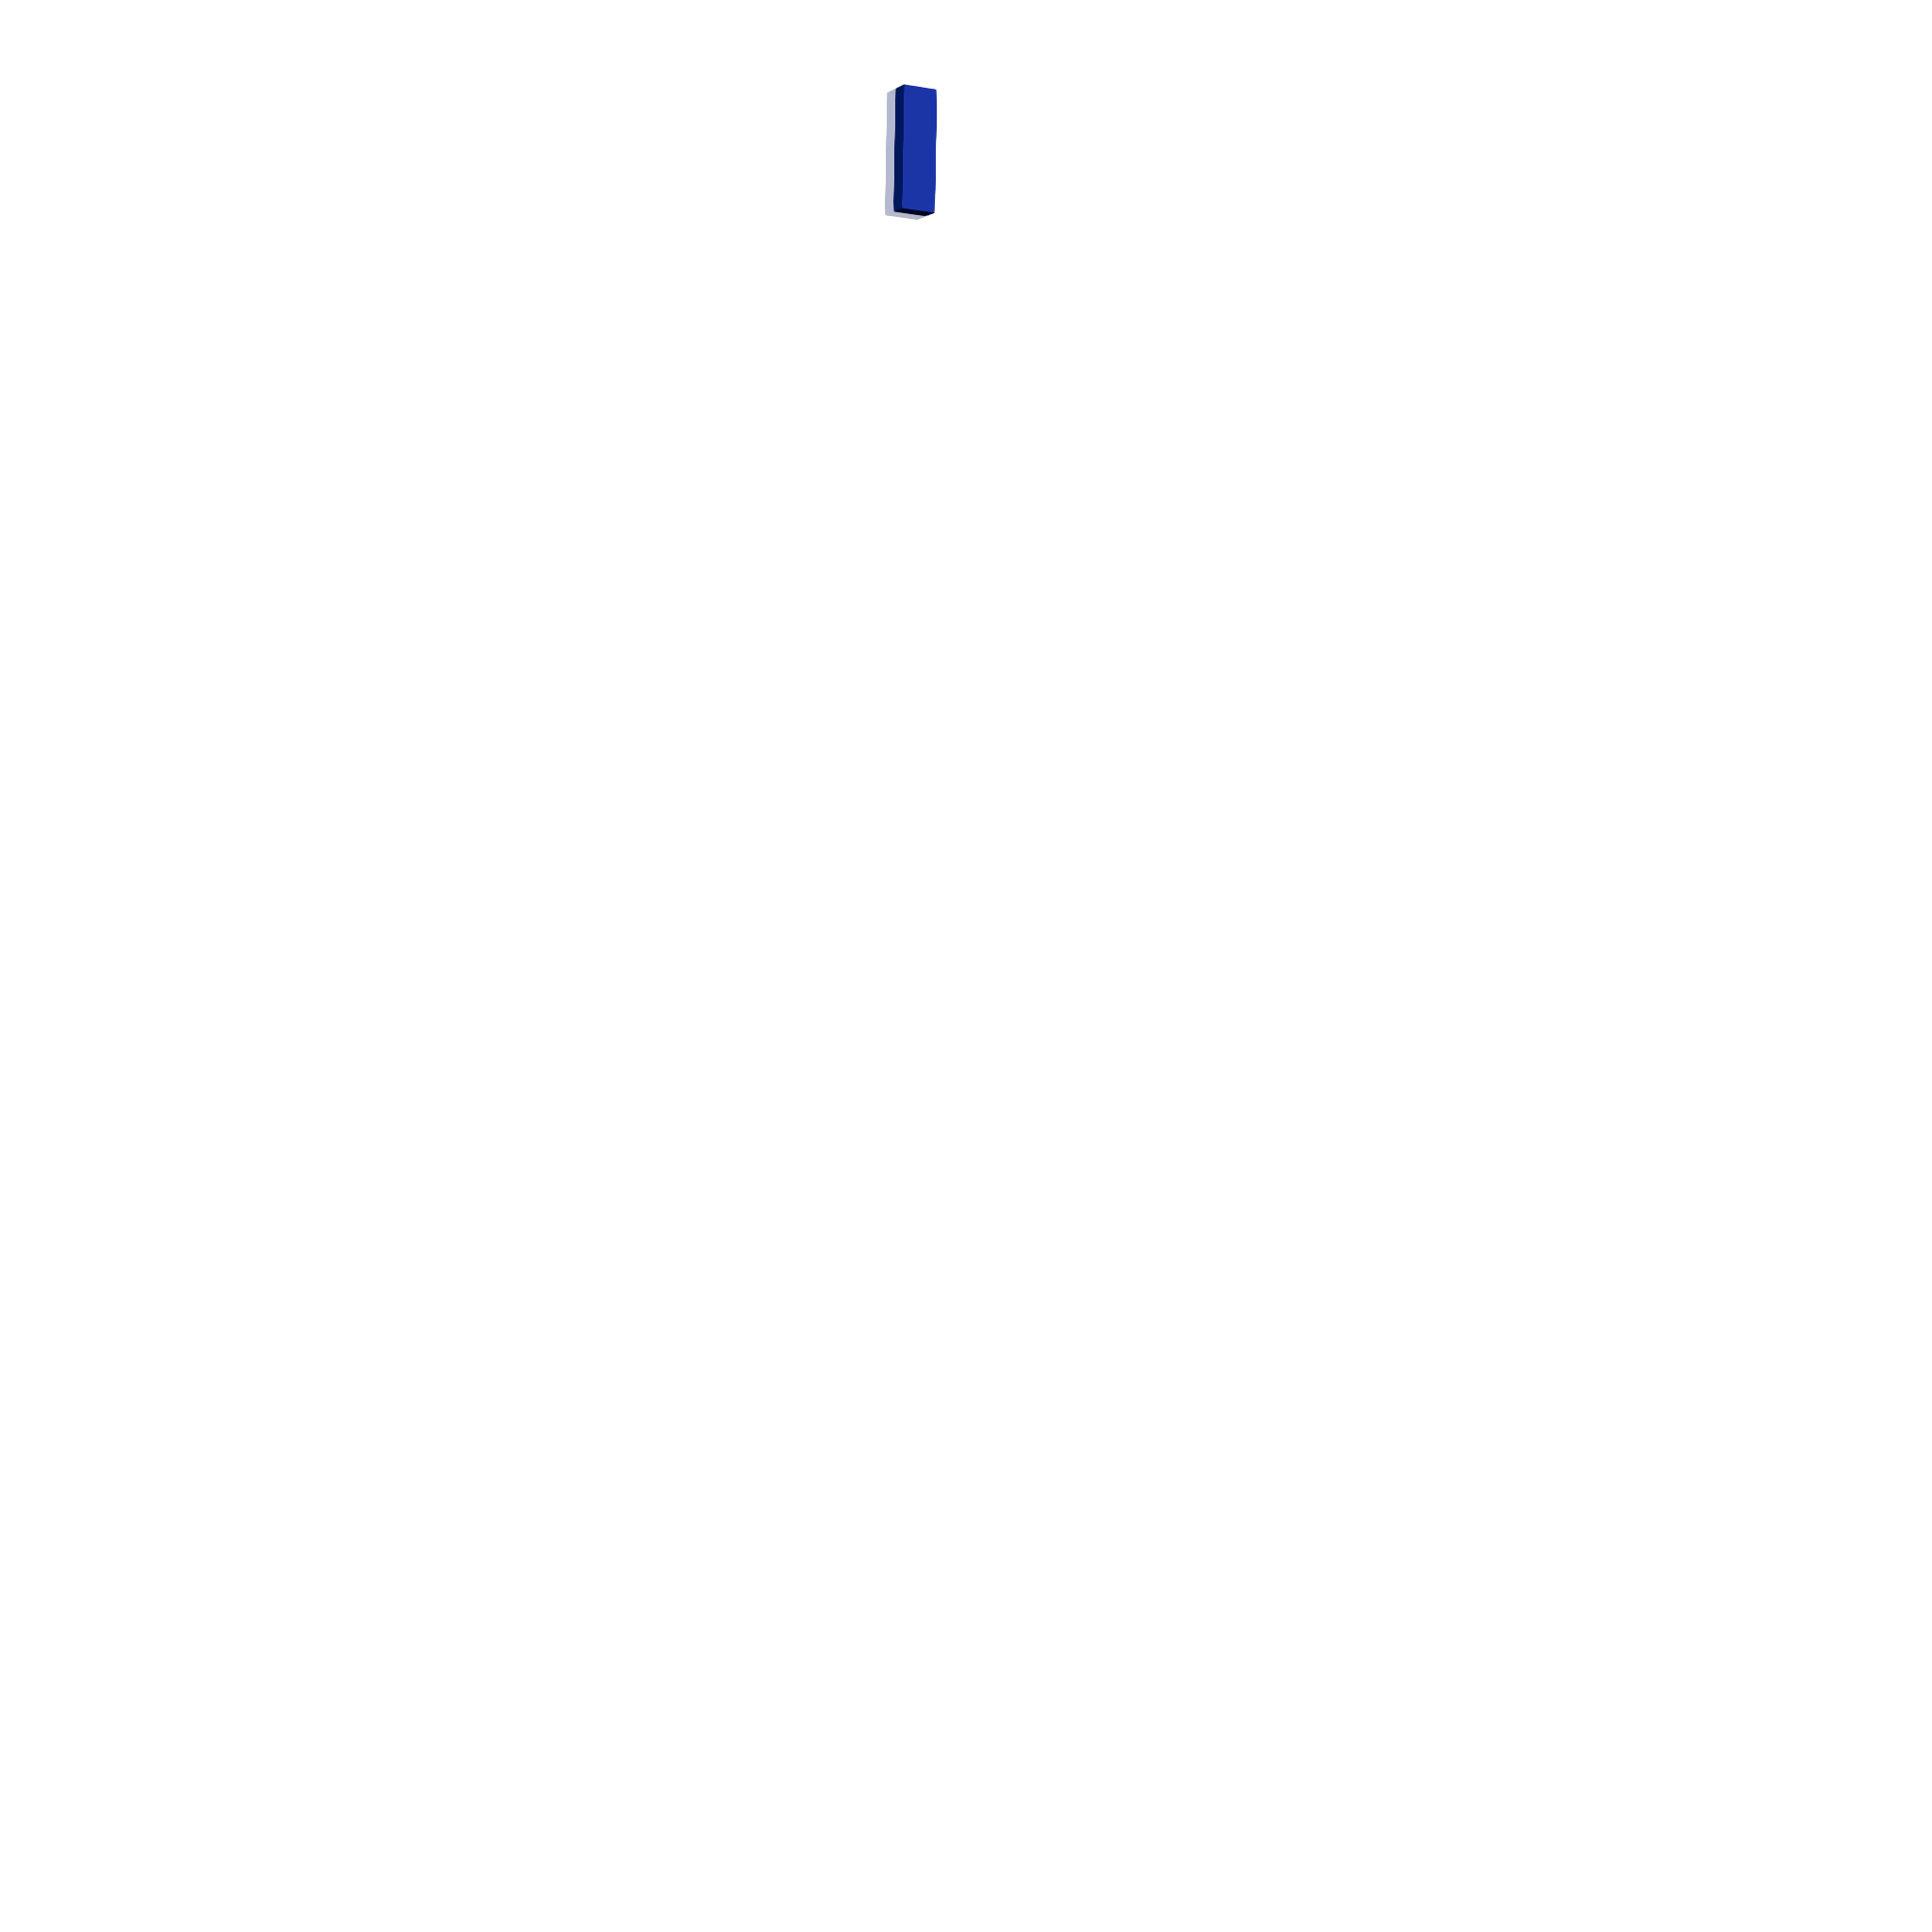
\includegraphics[width=0.333\textwidth]{figures/result_needle_0.png}}}
	\subfloat[Рост канала]{\frame{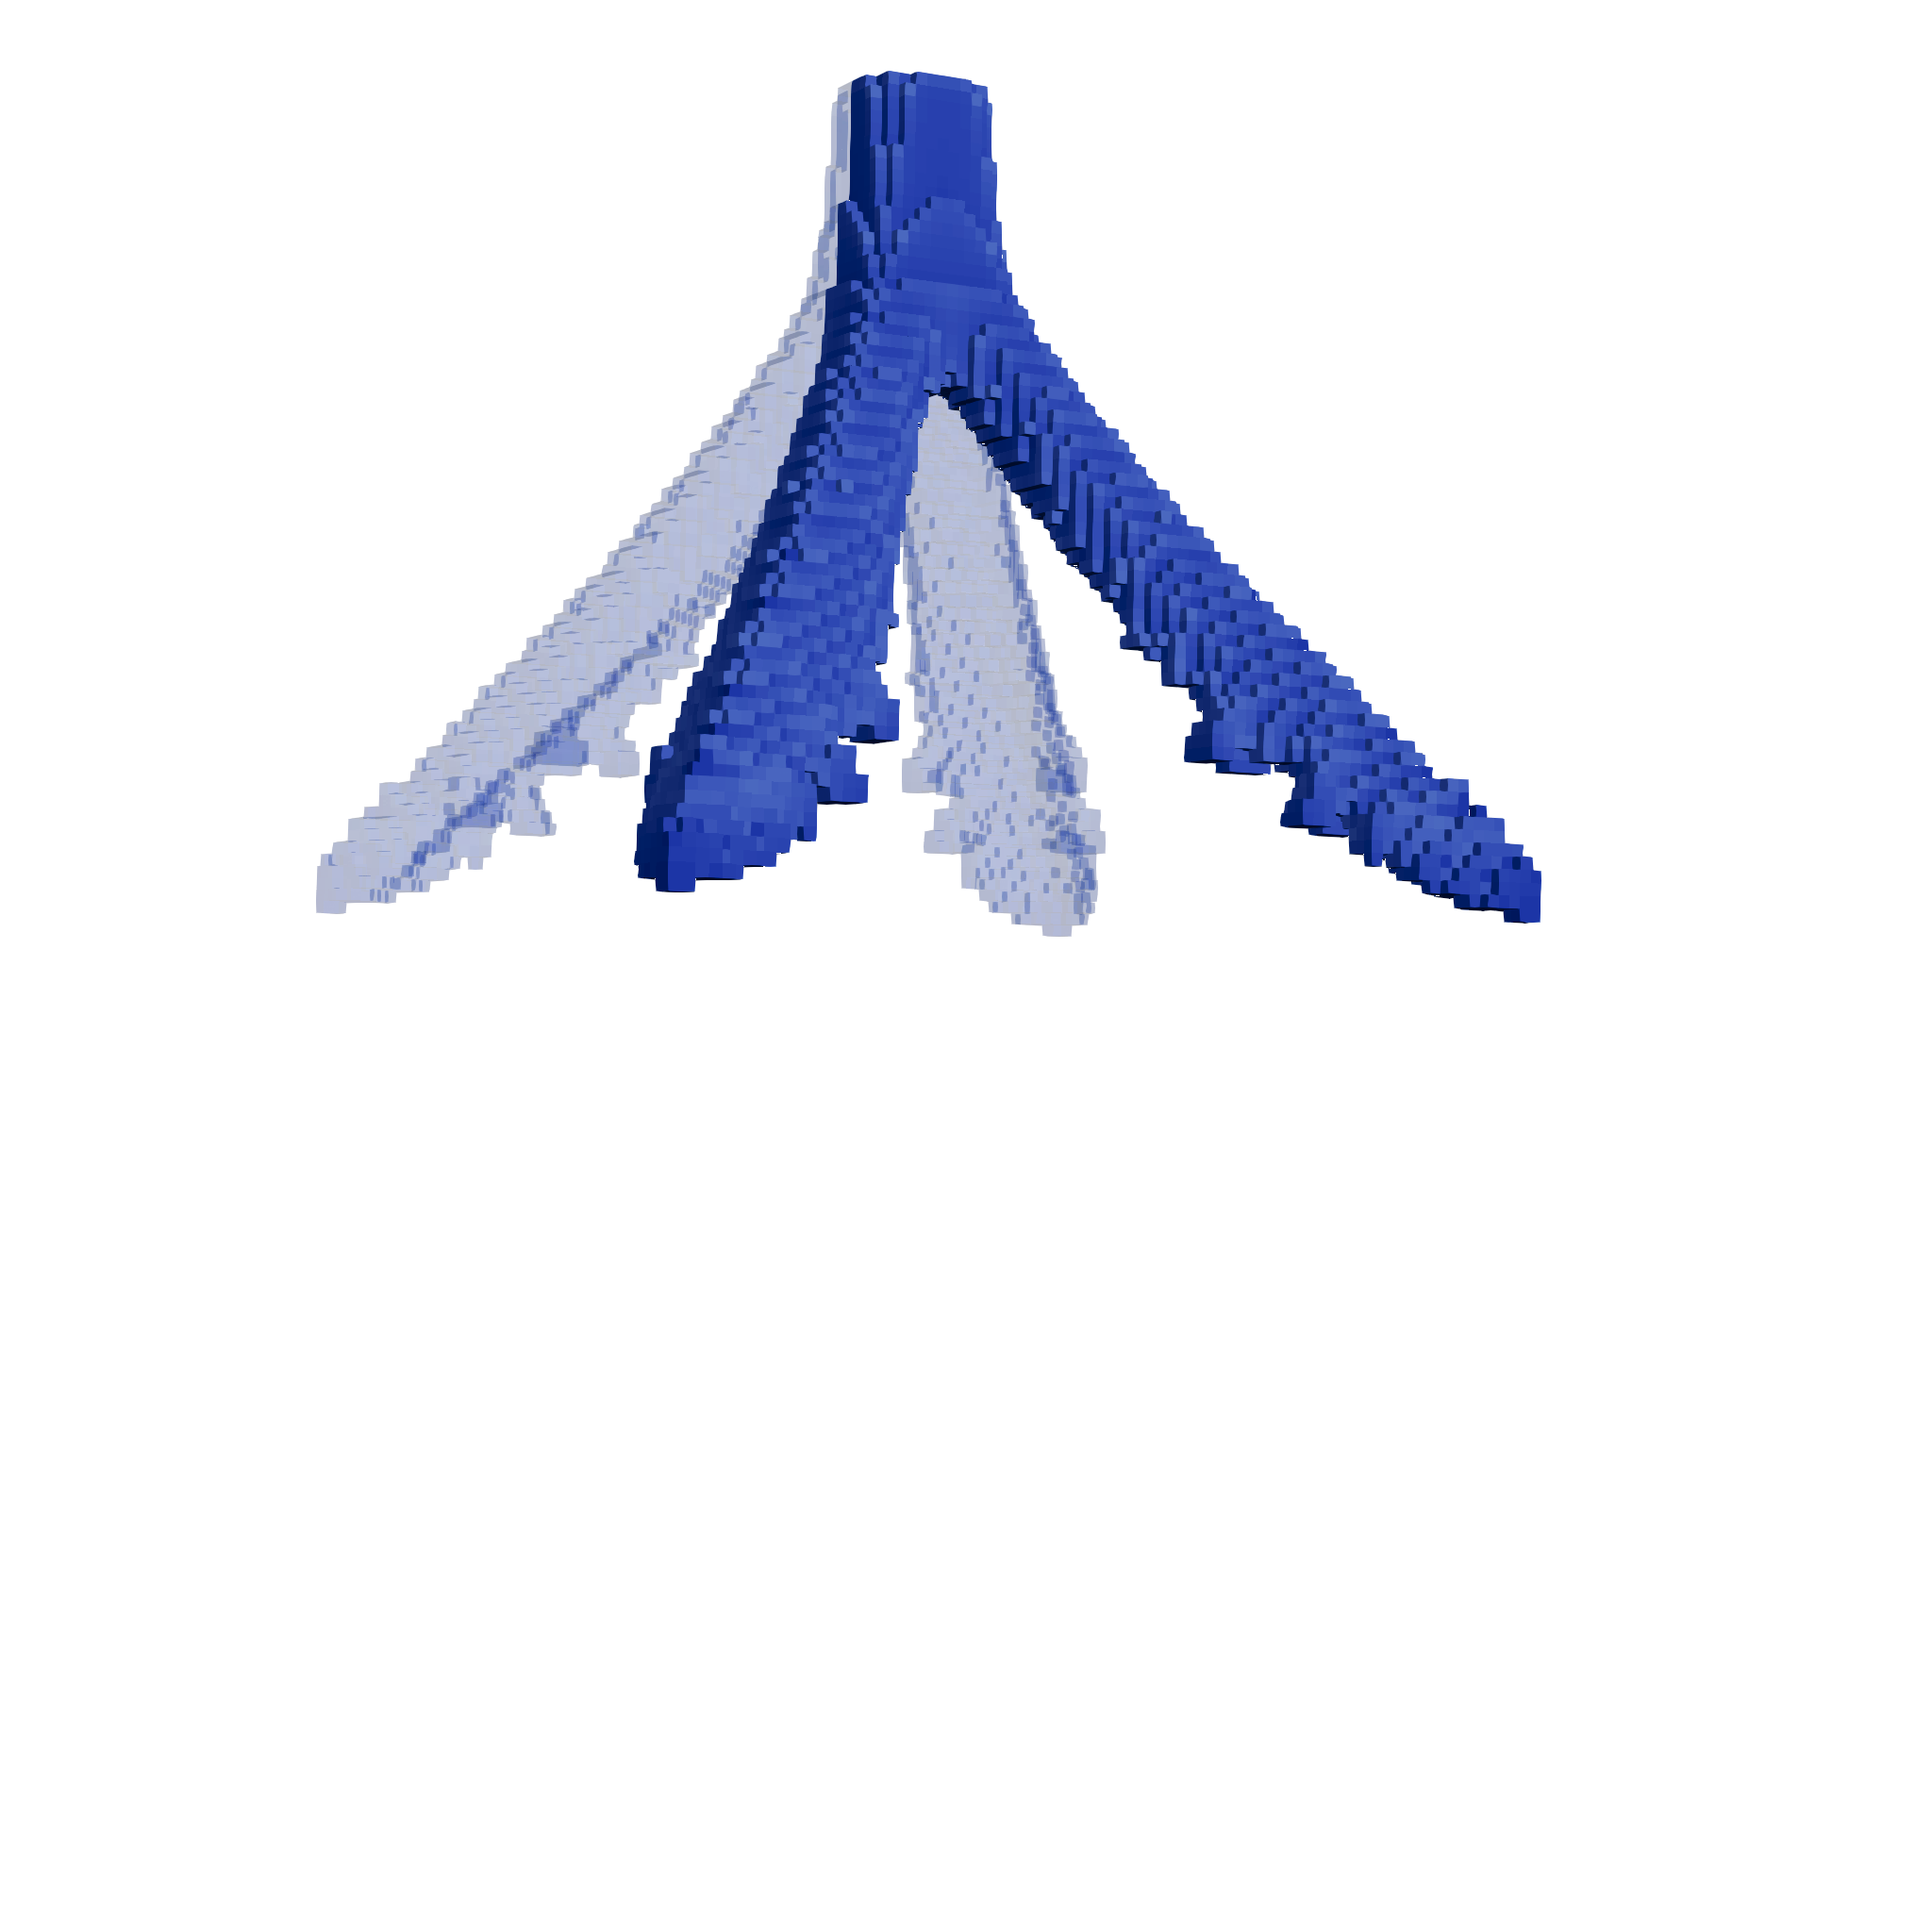
\includegraphics[width=0.333\textwidth]{figures/result_needle_1.png}}}
	\subfloat[Перед пробоем <<насквозь>>]{\frame{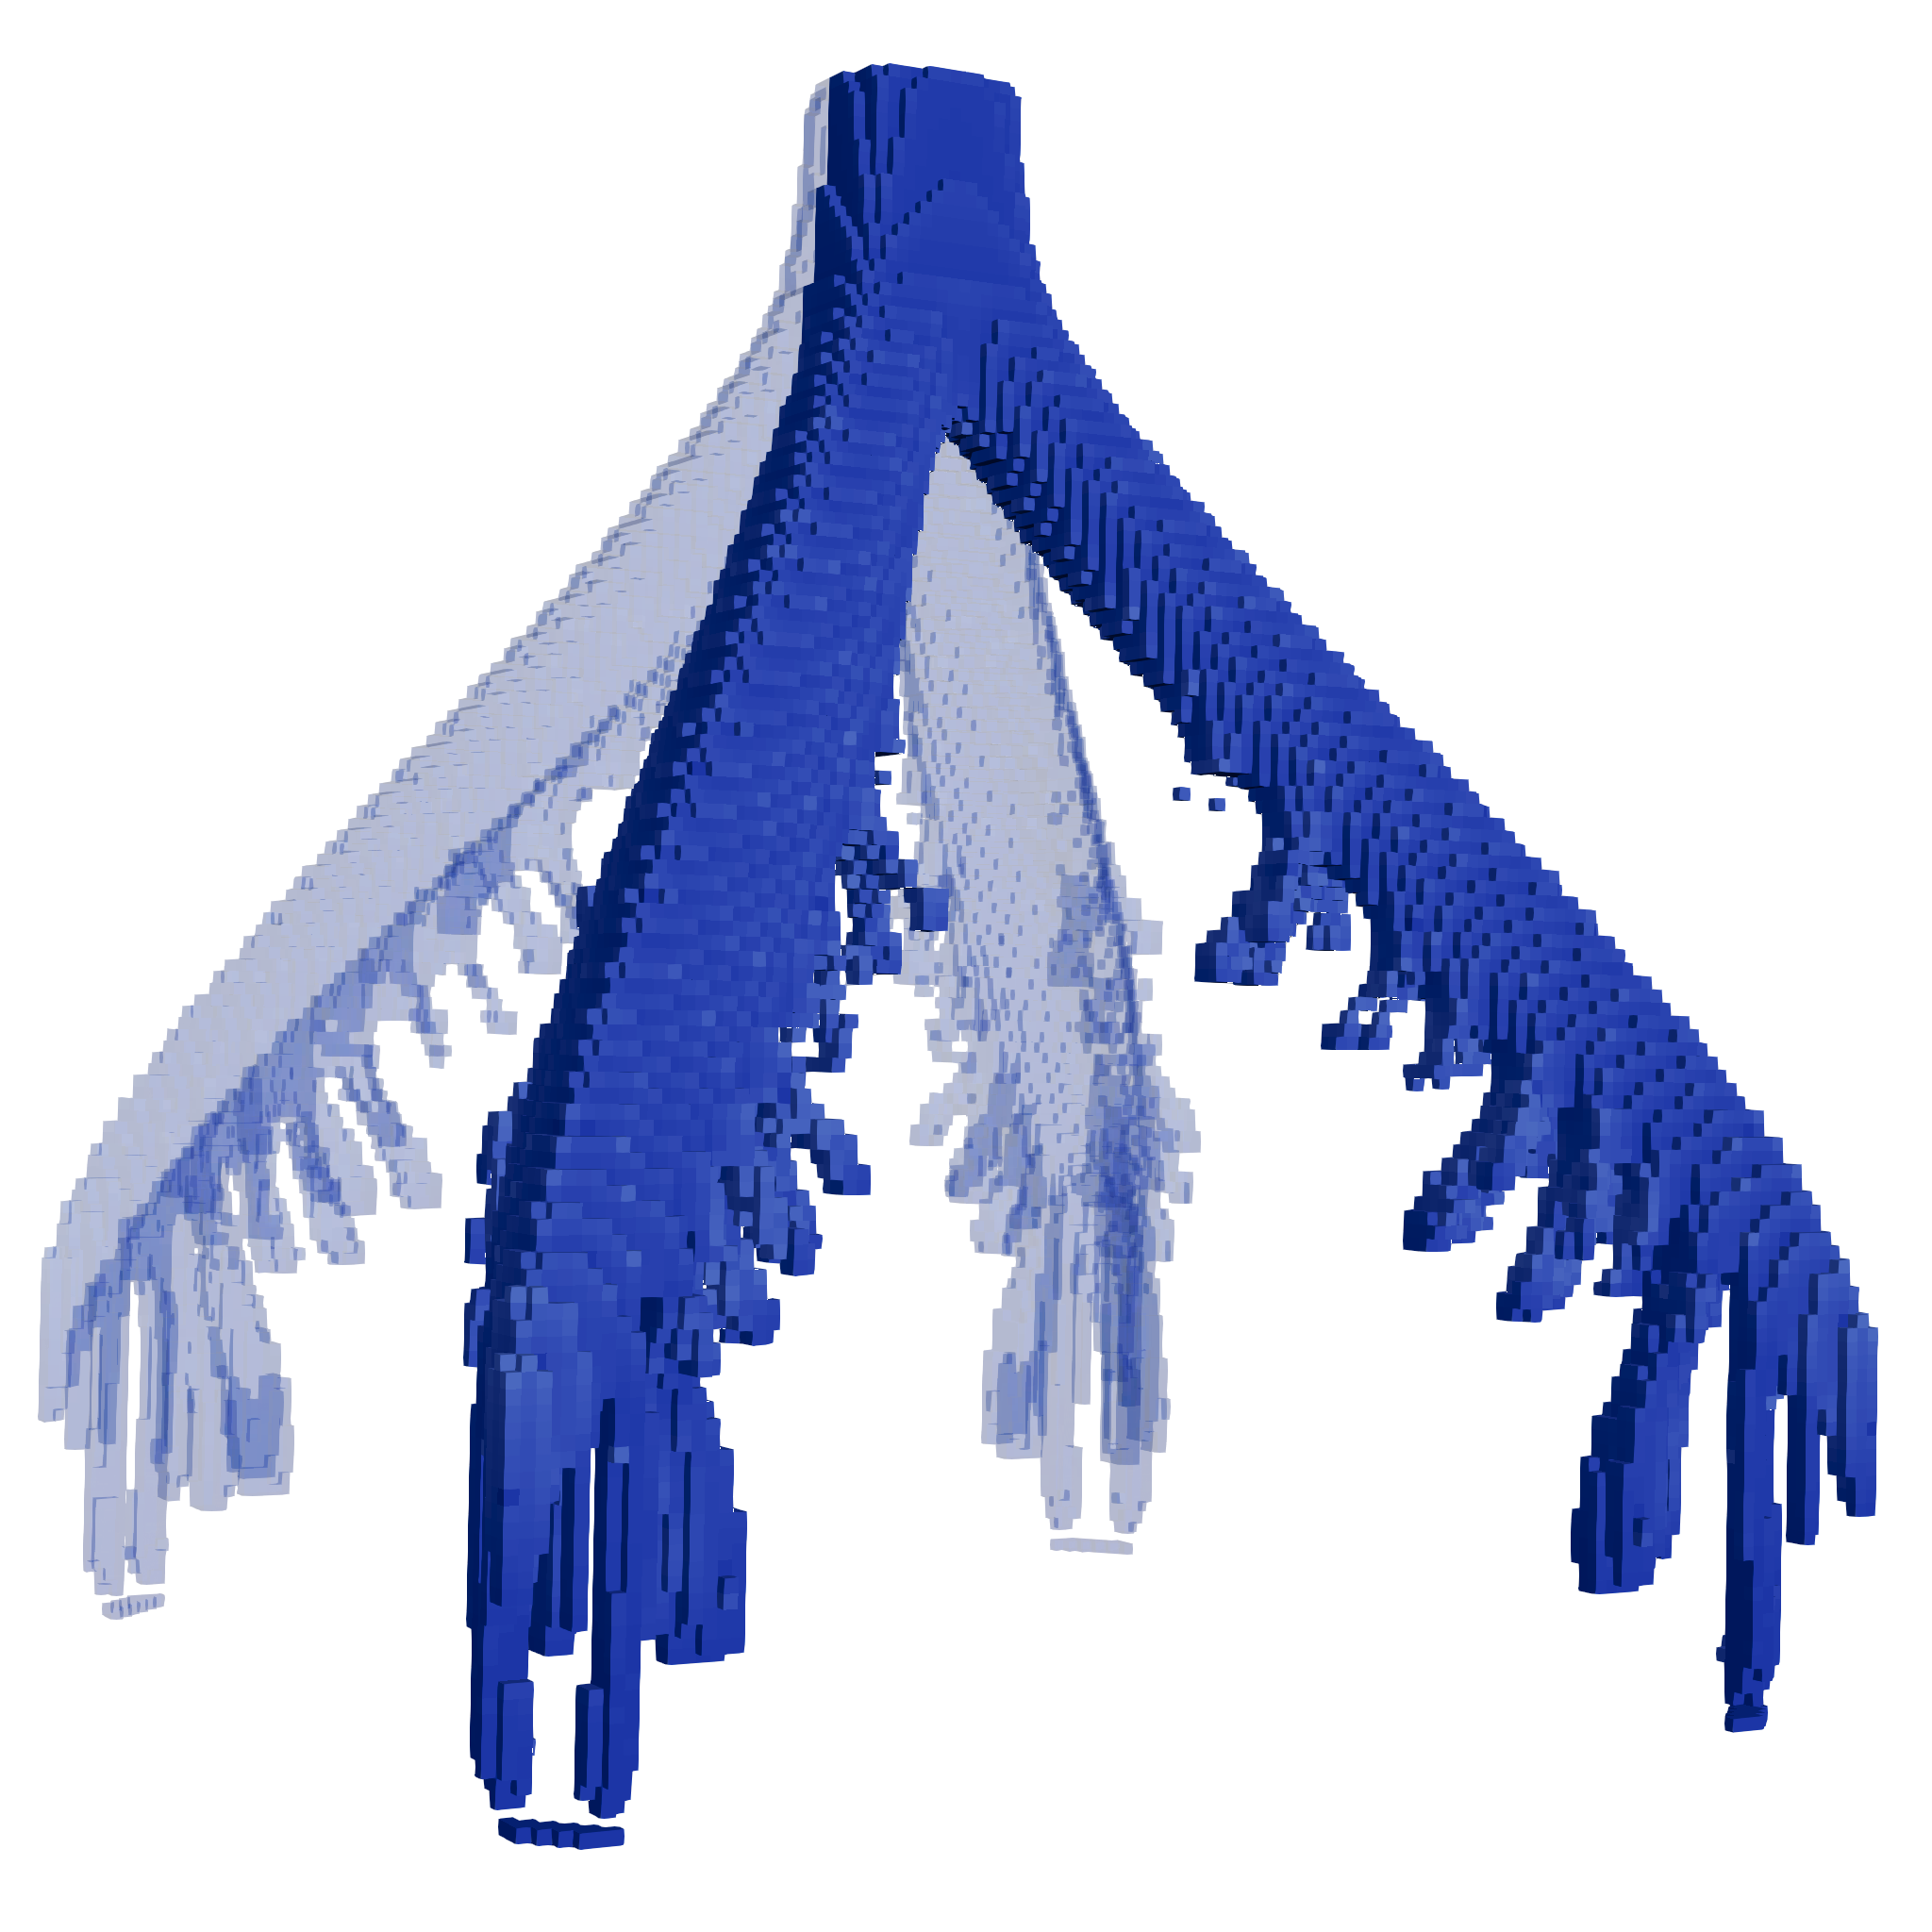
\includegraphics[width=0.333\textwidth]{figures/result_needle_2.png}}}
\end{figure}
\vspace{-7mm}
\begin{minipage}[l]{0.66\textwidth}
\begin{align*}
	N_h &= 129 & T &\approx 7 \cdot 10^{-7} & \taumin &= 10^{-12} \\
	N_t &= 51000 & \Tol &= 10^{-2} & \taumax &= 10^{-7}
\end{align*}
\end{minipage}
\end{frame}


\begin{frame}{Расчет №2: случайные возмущения}
\vspace{-5mm}
\begin{figure}
	\subfloat[Зародыши каналов]{\frame{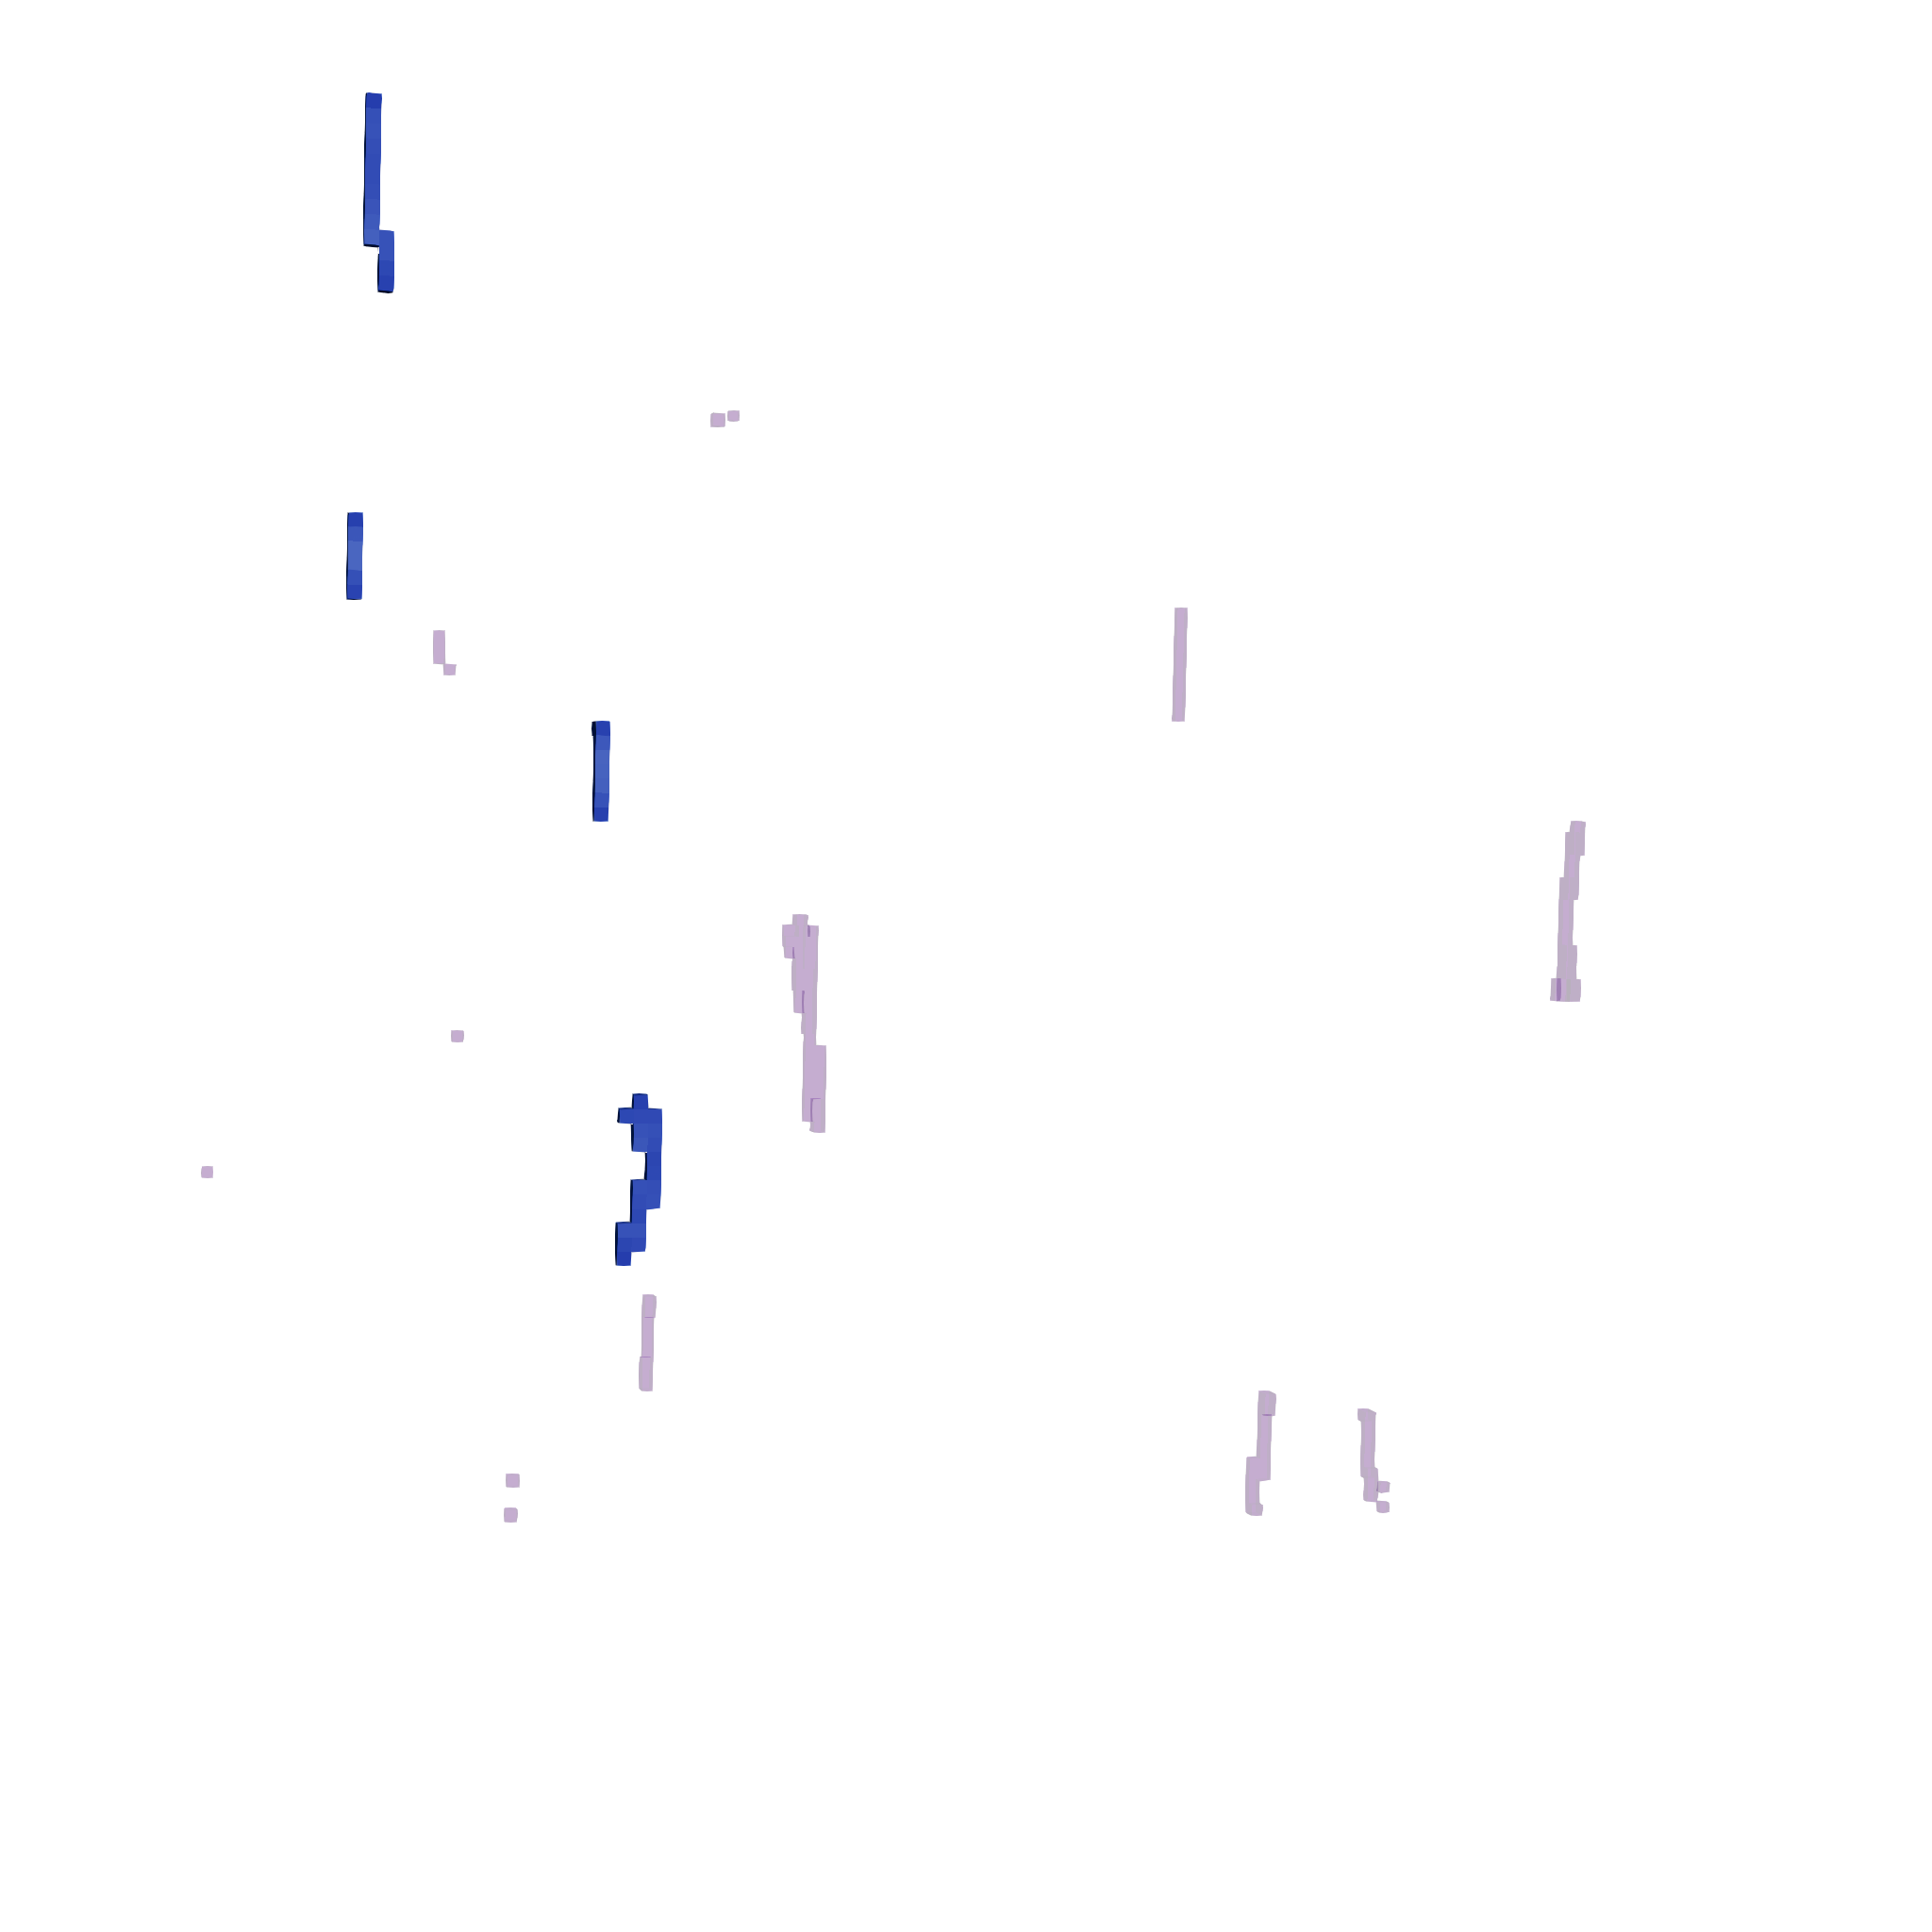
\includegraphics[width=0.333\textwidth]{figures/result_disturbance_1.png}}}
	\subfloat[Рост и слияние]{\frame{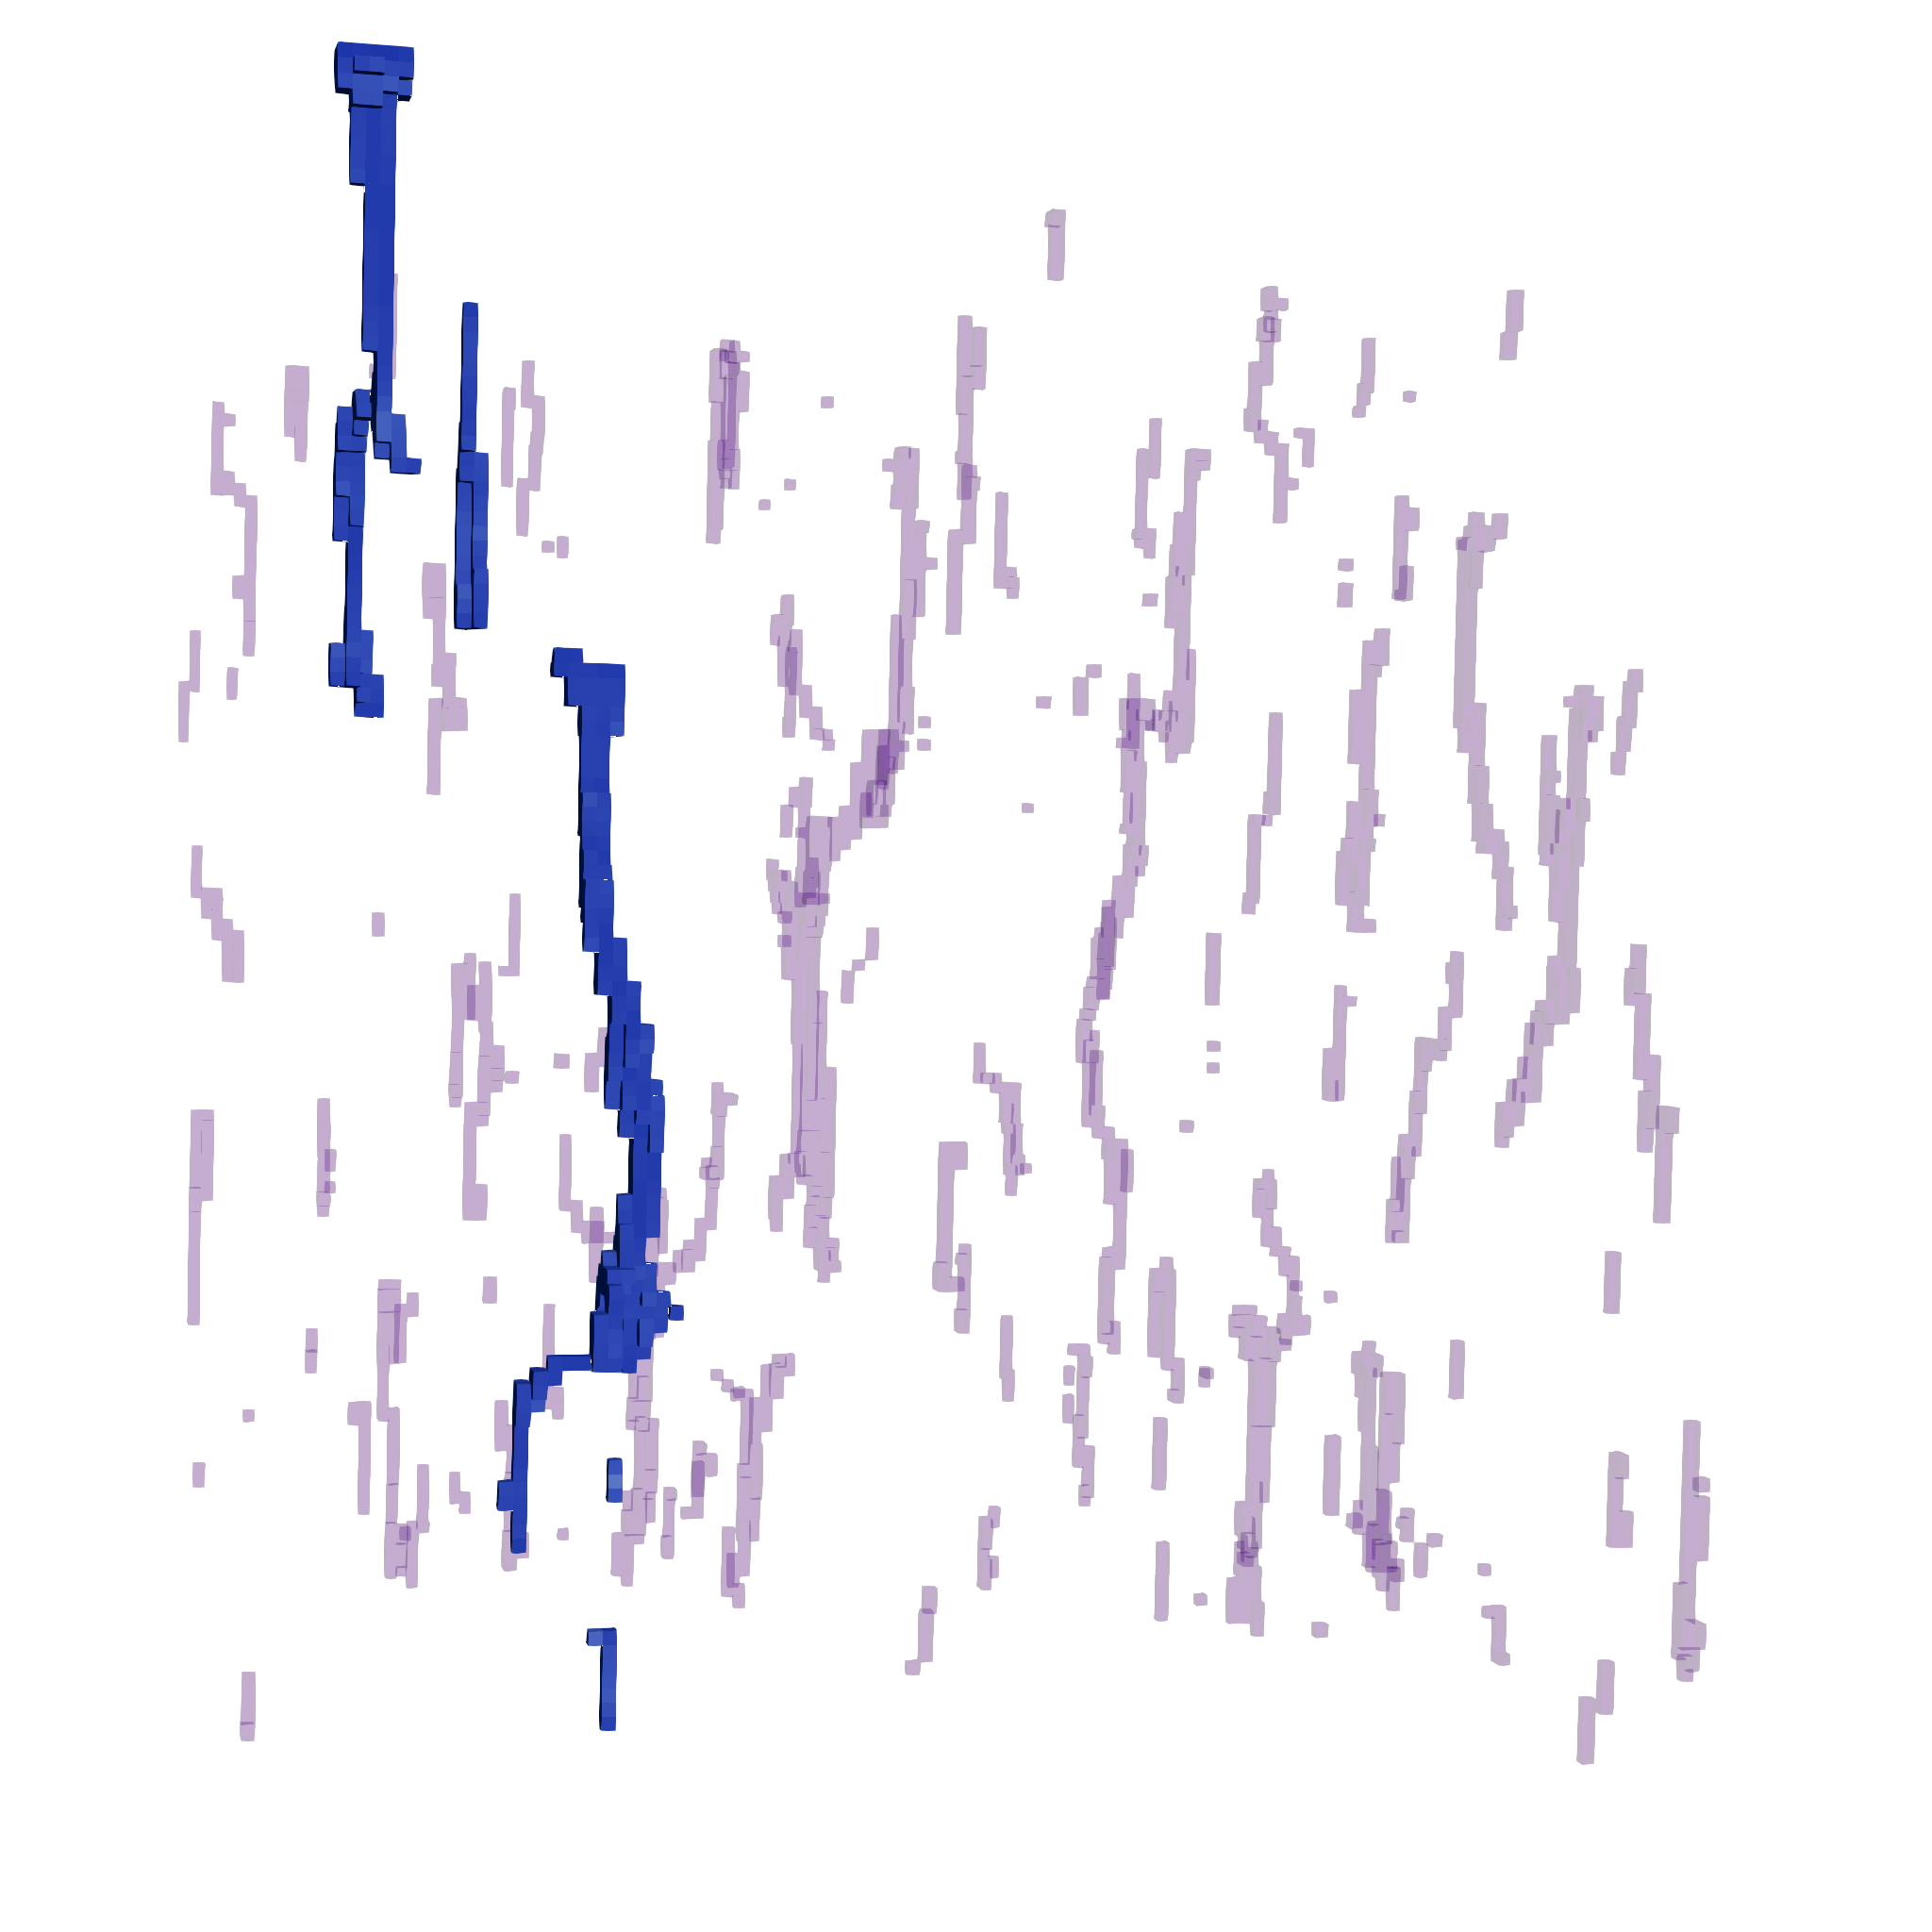
\includegraphics[width=0.333\textwidth]{figures/result_disturbance_2.png}}}
	\subfloat[Пробой <<насквозь>>]{\frame{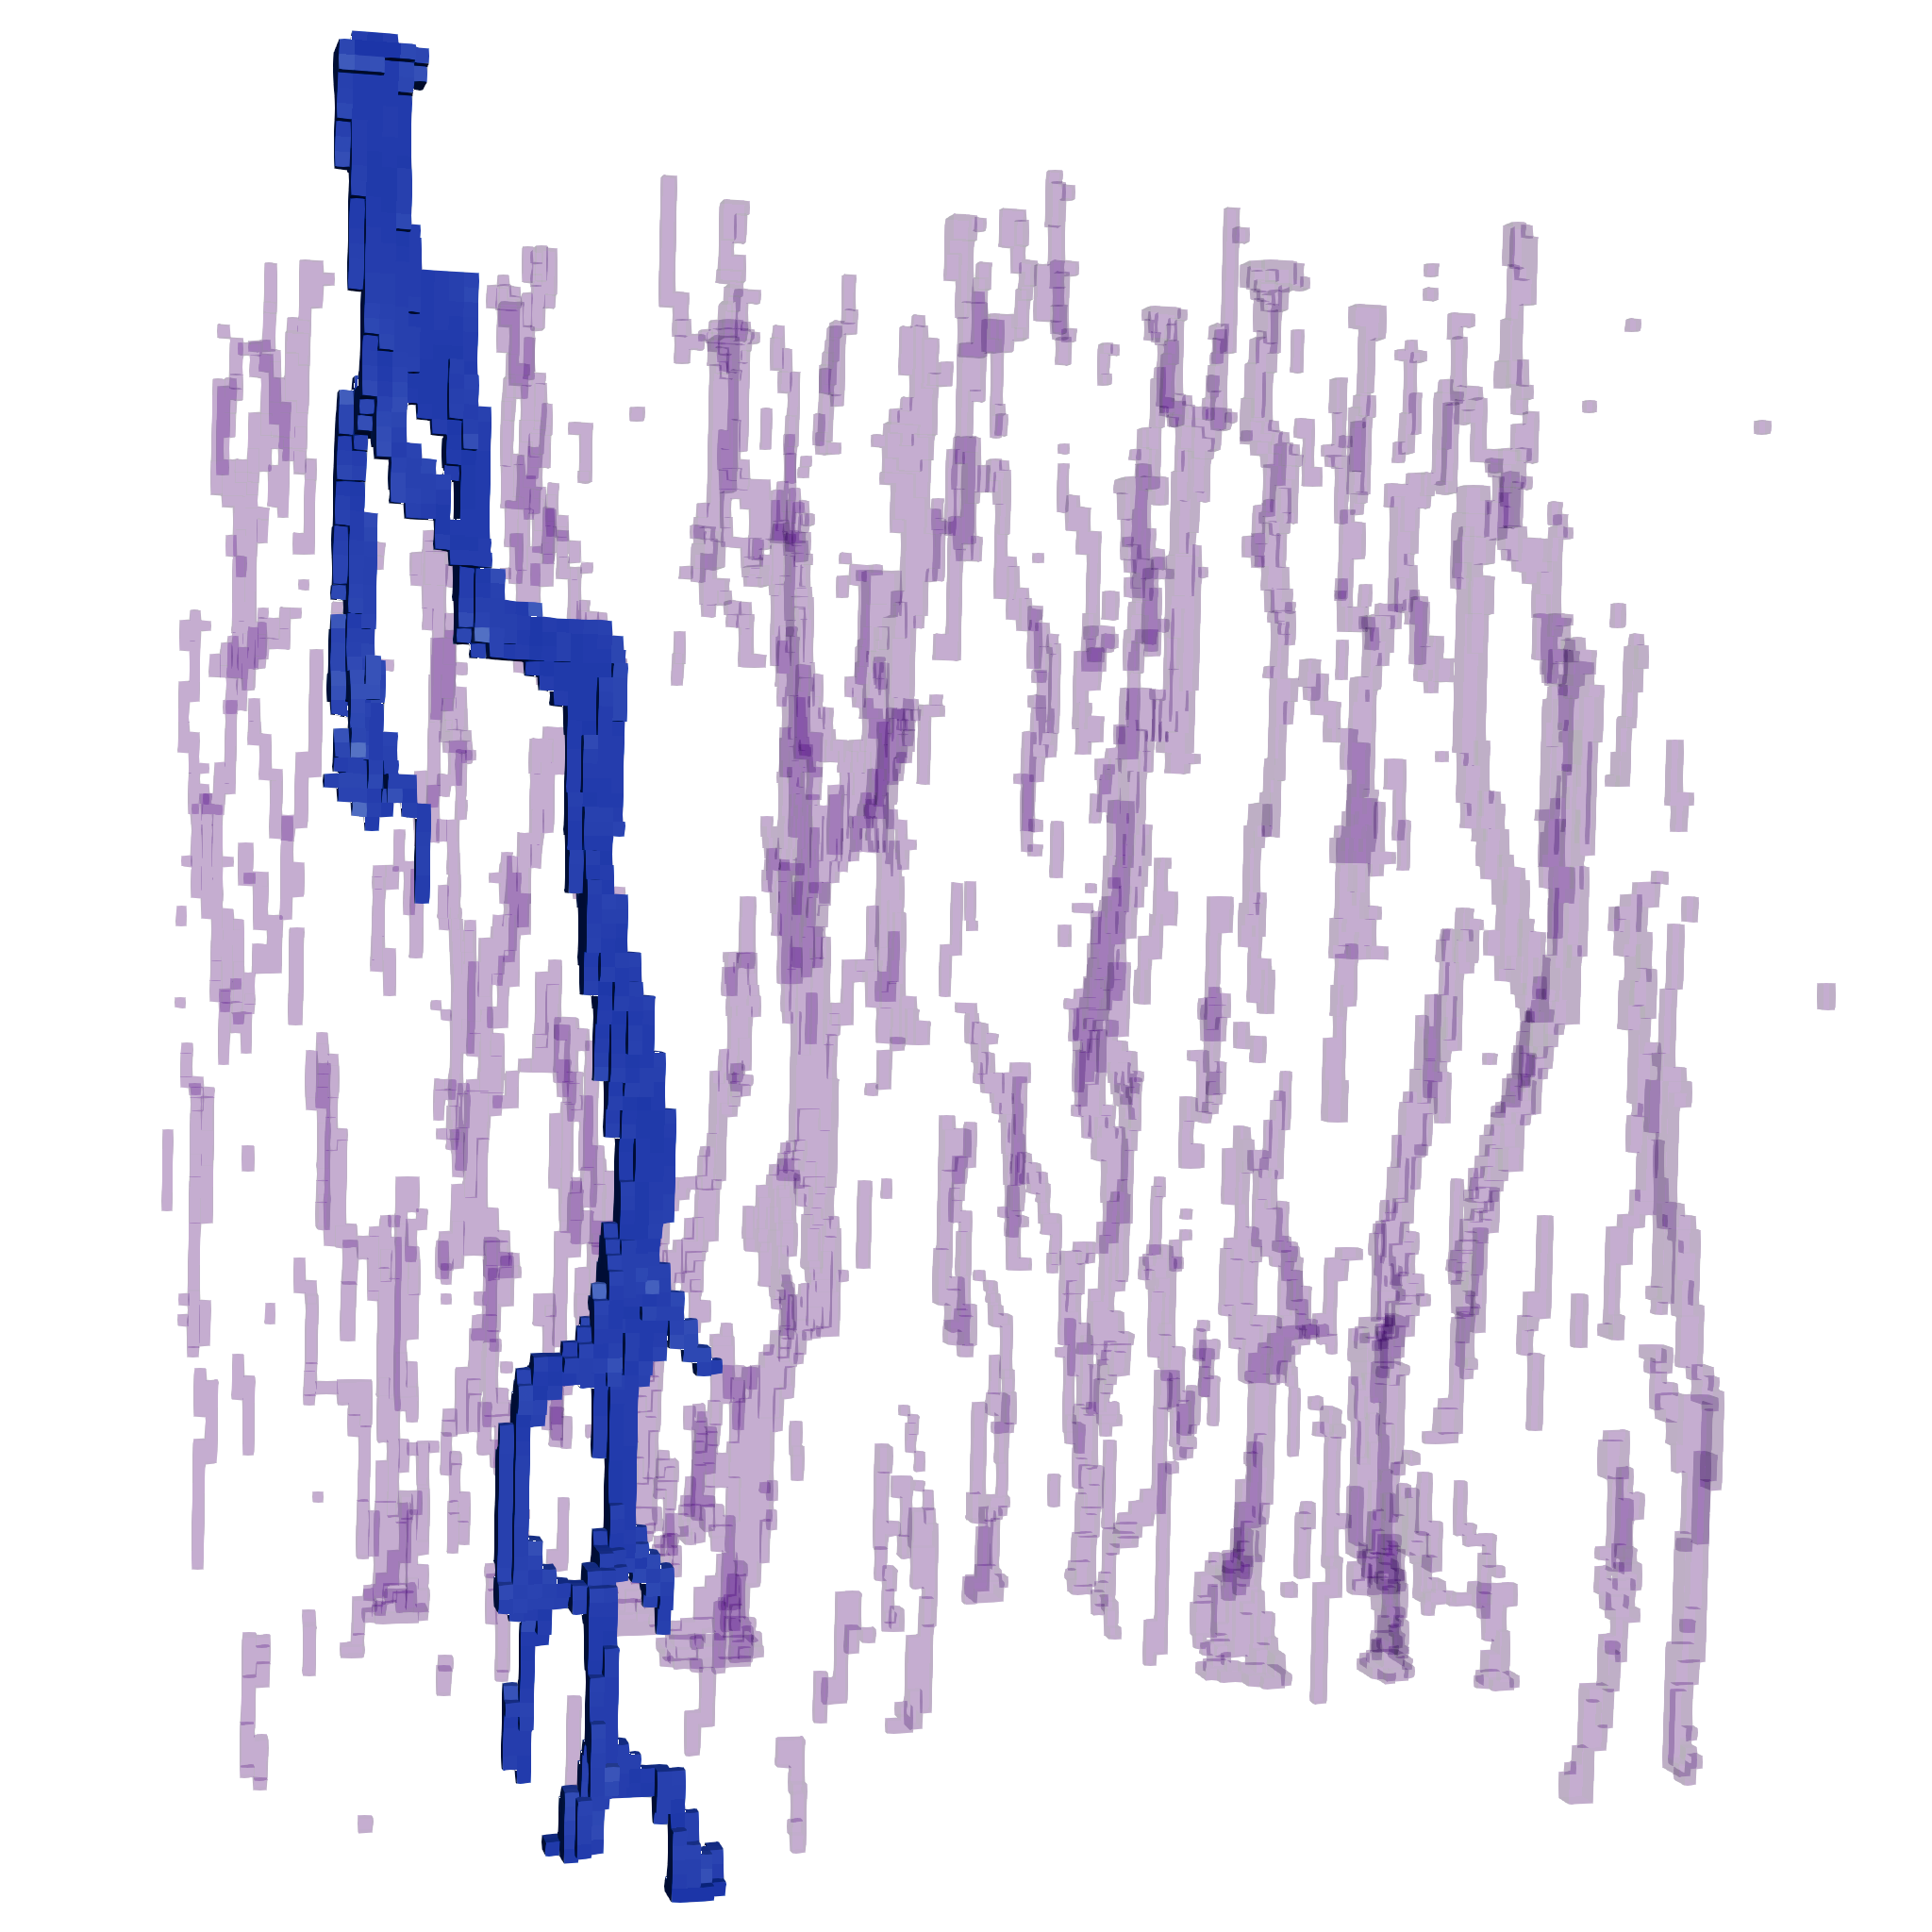
\includegraphics[width=0.333\textwidth]{figures/result_disturbance_3.png}}}
\end{figure}
\vspace{-7mm}
\begin{minipage}[l]{0.66\textwidth}
\begin{align*}
	N_h &= 129 & T &\approx 1.7 \cdot 10^{-6} & \taumin &= 10^{-12} \\
	N_t &= 22000 & \Tol &= 10^{-2} & \taumax &= 10^{-7}
\end{align*}
\end{minipage}
\end{frame}